\chapter{Analytic model of nondegenerate internal squeezing} %Research chapter: ...
\label{chp:nIS_analytics}

% results: interpret deep and far, and be very critical of assessing your approach
% present analysis of model and decisions/approximations made
% think about the story!
% systematic and diligent
% wring all of the information out of the results/figures, find the importance and the physics
% if you don't know, then justify your best guess with evidence

% separate this into multiple .tex files once structure finalised

%%%%%%%%%%%%%%%%%%%%%%%%%%%%%%%%%%%%%%%%%%
% chapter introduction

\jam{(Fix up mentions of nondegenerate internal squeezing in background chapters, either explain it earlier or do not confuse the reader)}

% combine the all-optical approach of dIS with the mode structure of sWLC
In this chapter, I present my analytic, Hamiltonian model of nondegenerate internal squeezing and discuss its immediate results.
%Nondegenerate internal squeezing is the same configuration as degenerate internal squeezing except that the squeezer is operated nondegenerately, but it is better thought of as an all-optical alternative to stable optomechanical filtering.
Firstly, I will describe nondegenerate internal squeezing and how it is motivated by the existing proposals in the previous chapter. Secondly, I will present my model to derive the sensitivity of the configuration. I will characterise the sensitivity, partially verify the model by demonstrating that it obeys the expected low and high loss limits, and show that the system is stable. Finally, I will find the squeezing threshold of nondegenerate internal squeezing using an observation about its stability. % that unites the different squeezing configurations in this thesis. 
% from the view of quantum optics, gravitational waves in the next chapter
This chapter is directed at understanding nondegenerate internal squeezing for general quantum metrology. In the following chapters, I will return to the problem of kilohertz gravitational-wave detection and whether nondegenerate internal squeezing can feasibly improve sensitivity. 


\section{Motivation from existing proposals}
% Conceptual understanding and relation to existing proposals
\label{sec:modal_equivalence}

\begin{figure}
    \centering
    \includegraphics[angle=-90,width=0.7\textwidth]{nIS_mode_diagram.pdf}
    % squeezing ellipse and signal arrow plot
    \caption{\jam{(Purpose: explain configuration)} Nondegenerate internal squeezing's mode diagram (top panel) and simplified effect on the signal and noise (bottom panel). The core system consists of three coupled, optical modes $\hat a,\hat b,\hat c$. The gravitational-wave signal couples through them and is measured in the signal and/or idler mode at the photodetector. Optical losses and the pump mode are omitted from the mode diagram. Compare the mode diagram to degenerate internal squeezing and stable optomechanical filtering in Fig.~\ref{fig:mode_diagram}. The system's simplified response is shown using the signal arrow and noise ellipse representation from Fig.~\ref{fig:extSqz_config}. The noise is anti-squeezed but the gravitational-wave signal is amplified more such that the sensitivity improves.}
    \label{fig:nIS_mode_diagram}
\end{figure}
\begin{figure}
    \centering
    \includegraphics[width=0.7\textwidth]{all_mode_structures.pdf}
    \caption{Simplified mode diagrams of the OPOs, degenerate internal squeezing, stable optomechanical filtering, and nondegenerate internal squeezing. The modes and coupling rates are explained in the text. Whenever the arm mode $\hat a$ is shown, it is implicitly connected to the test mass mechanical mode $\hat x$ and the gravitational wave signal $h(t)$. The parallels between the degenerate OPO and degenerate internal squeezing, and the nondegenerate OPO and nondegenerate internal squeezing can be seen. Nondegenerate internal squeezing and stable optomechanical filtering are modally equivalent but are optomechanical and all-optical, respectively, which means that their performance might be different given the different losses they encounter. Idler readout of the mechanical idler mode is more difficult but potentially possible~\cite{liEnhancingInterferometerSensitivity2021}.}
    \label{fig:mode_diagram}
\end{figure}

Nondegenerate internal squeezing consists of a nondegenerate squeezer placed inside the signal-recycling cavity of an interferometer~\cite{}. It is the same configuration as degenerate internal squeezing, shown in Fig.~\ref{fig:dIS_config}, except that the squeezer is operated nondegenerately -- like the relation between the nondegenerate and degenerate OPOs. The general idea being to instead anti-squeeze the noise but amplify the signal more, as shown in the bottom panel of Fig.~\ref{fig:nIS_mode_diagram}, which motivates investigating nondegenerate internal squeezing since this might make it more resistant to optical loss than degenerate internal squeezing because the loss will instead decrease the noise to the vacuum value. %by the same argument as Section~\ref{sec:cavess_amp}. %However, it is better thought of as an all-optical alternative to stable optomechanical filtering, which I will show.
The mode structure of nondegenerate internal squeezing in the single-mode approximation is shown in the top panel of Fig.~\ref{fig:nIS_mode_diagram}, where the signal and idler modes are resonant in the signal-recycling cavity but the signal mode $\hat b$ at $\omega_0$ is resonant in the arms while the idler mode $\hat c$ at $\omega_0+\Delta$ is not resonant in the arms, such that the arm $\hat a$ and idler $\hat c$ modes are not directly coupled. I compare this mode structure to the existing proposals and the OPOs in Fig.~\ref{fig:mode_diagram}, which shows that, although it might initially sound closer to degenerate internal squeezing, nondegenerate internal squeezing is equivalent to stable optomechanical filtering under the mapping of the optical idler mode $\hat c$ at $\omega_0+\Delta$ and squeezer parameter $\chi$ to the mechanical idler mode $\hat{c}_m$ at $\omega_m$ \jam{(is this greater than $\omega_0$?)} and optomechanical coupling $\chi_m$, respectively, in the Hamiltonian~\cite{liBroadbandSensitivityImprovement2020}. In this sense, it is an all-optical analogue of the optomechanical configuration.
However, although the Langevin terms~\cite{} describing the associated optical and mechanical loss and quantum and thermal noise, respectively, of the all-optical and optomechanical analogues are also equivalent under a similar mapping~\cite{}, the two lossy configurations are not equivalent because of the different realistic levels of optical and mechanical loss~\footnote{Although, because the mechanical loss dominates the optomechanical analogue, I expect the optical idler loss to dominate nondegenerate internal squeezing.}. This motivates investigating nondegenerate internal squeezing since it might have similar sensitivity improvement as the optomechanical analogue but have more realistic loss requirements. % than the mechanical loss required for the optomechanical analogue.
% \jam{(different experimental constraints on optical loss versus mechanical loss?)}

% \jam{(Should this literature review be merged with the others?)}
% This modal equivalence~\cite{liBroadbandSensitivityImprovement2020} is the only direct mention of nondegenerate internal squeezing in the literature \jam{(that I could find, check this!)}. 
 % which I attribute to the recency~\cite{korobkoQuantumExpanderGravitationalwave2019,liBroadbandSensitivityImprovement2020} of the two existing proposals in the previous chapter which motivate it.
% In the work studying the optomechanical analogue~\cite{liBroadbandSensitivityImprovement2020,liEnhancingInterferometerSensitivity2021}, only mechanical loss is included in the model \jam{(check Li2021)} since it is the dominant source of loss, but a full understanding of the system requires all realistic optical losses to be included \jam{(quantify difference?)}. % at the realistic levels for a future detector. % -- rather than indirectly by considering realistic mechanical losses. 
% Therefore, I identify this as a gap in the literature, no work has fully characterised nondegenerate internal squeezing with realistic optical loss in every mode to determine its feasibility for detection.
% Moreover, other aspects of the system are also not known, such as its low and high loss limits and lossy threshold. I partially fill this gap in this thesis. 

% all-optical alternative
% Finally, there is an alternative route to progress, to replace the optomechanical interaction with an all-optical one and replace the mechanical loss with optical loss. This is to consider nondegenerate internal squeezing, where the internal squeezer squeezes signal and idler modes and the idler is not resonant in the arms~\footnote{So that the idler mode is not coupled to the arm cavity mode.}. 
% although nIS is closer on first inspection to dIS, the underlying structure is closer to sWLC, but both motivate it.
% equivalent mode structures, just the different noise sources
% Although it might seem closer to degenerate internal squeezing than stable optomechanical filtering, the underlying mode structure of nondegenerate internal squeezing is equivalent to the latter, by mapping the idler optical mode and squeezer parameter $\hat c, \chi$ to the mechanical mode and optomechanical coupling $\hat{c}_m, \chi_m$, respectively, in the Hamiltonian~\cite{}, as shown in Fig.~\ref{fig:mode_diagram}.
% Although this is only true in the case with no optical or mechanical loss, as thermal noise in $\hat{c}_m$ behaves differently to shot noise in $\hat c$~\cite{} \jam{(it does experimentally and the parameter regimes are very different in application, but the Langevin terms are the same)}, it is reasonable to predict that the lossy configurations behave similarly to each other because the abstract dynamics are the same. Therefore, nondegenerate internal squeezing might achieve the sensitivity improvement of stable optomechanical filtering but at more realistic optical loss than the mechanical loss required above.

% \section{Literature review}
% a gap in the literature, should be much shorter than the review in Section~\ref{sec:literature_review} -- maybe combine it with that one?
% cannot cite personal communication?
% claim: the modelling of this configuration has never been done as thoroughly as my work, explain why (recency of interest)

% \jam{(How to be thorough with this section?)}
% The available literature on nondegenerate internal squeezing is limited. Although nondegenerate OPOs have long been studied for tests of the EPR-paradox~\cite{Reid1989,Schori2001} and other applications~\cite{,,}, placing a nondegenerate squeezer in a coupled cavity system \jam{has only been studied in ... (I am not aware of any other mentions than liBroadbandSensitivityImprovement2020, ask the supervisors.)}. 
% Although nondegenerate internal squeezing is motivated by the two configurations in the previous chapter, those configurations have only been studied in the last few years, see Section~\ref{sec:literature_review}. \jam{(Is there direct mention of nIS in the dIS literature?)}
% The only direct mention of nondegenerate internal squeezing \jam{(that I could find, check this!)} in the literature is the brief suggestion in Ref.~\cite{liBroadbandSensitivityImprovement2020} that it is equivalent to stable optomechanical filtering in the lossless case. In that paper and subsequent work by the same authors~\cite{liEnhancingInterferometerSensitivity2021}, only mechanical loss is included in the model since it is the dominant source of loss. By the modal equivalence in Section~\ref{sec:modal_equivalence}, I predict that optical loss in the idler mode should be the dominant source of loss for nondegenerate internal squeezing but this is not known.
 % distribution of loss in applications might be far from uniform, e.g.\ how the detection loss is predicted to be higher than any of the intra-cavity losses for future gravitational-wave detectors~\cite{}.


\section{Analytic model}
\label{sec:nIS_model}

\begin{figure}
	\centering
	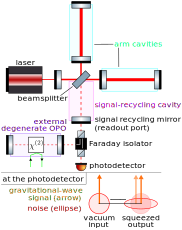
\includegraphics[angle=-90,width=0.9\textwidth]{nIS_config.pdf}
	\caption{\jam{(Purpose: explain configuration)} \jam{(Explain coupled-cavity approximation here, simplify loss ports s.t. linear cavities)} Nondegenerate internal squeezing configuration with all modes and losses labelled as explained in the text, compared to the mode diagram in Fig.~\ref{fig:nIS_mode_diagram}. The idler mode is not resonant in the arms and therefore the three modes are coupled as $\hat a$ to $\hat b$ to $\hat c$. The interferometer mirrors are labelled as the ETM (end test mass), ITM (input test mass), and SRM (signal-recycling mirror). The intra-cavity loss ports are shown as mirrors instead of beamsplitters but the model of optical loss is the same \jam{(update with reference to new figure)}. This combines the configurations of the nondegenerate OPO in Fig.~\ref{fig:OPOs_config}, degenerate internal squeezing in Fig.~\ref{fig:dIS_config}, and stable optomechanical filtering in Fig.~\ref{fig:sWLC_config}.}
	\label{fig:nIS_config}
\end{figure}

I model nondegenerate internal squeezing using the Hamiltonian method from Section~\ref{sec:Hamiltonian_modelling}. %, in particular, this model combines the nondegenerate OPO model in Section~\ref{sec:nOPO} and the ~\ref{sec:dIS_model}, respectively.
% There are no steps in this derivation that have not already appeared in this thesis \jam{(check this)}.
% This model is based on and verified against the lossless model for the optomechanical analogue in Ref.~\cite{liBroadbandSensitivityImprovement2020} which effectively couples an arm cavity mode to the nondegenerate OPO model in Section~\ref{sec:nOPO}. %, and to that model I add intra-cavity and detection losses.
% \jam{(Probably need to talk about my methodology more -- state that this derivation presented is the last of a long line of increasing complexity (more losses, radiation pressure, pump phase, etc.) and that I have verified at each stage that the model recovers the previous model. This allowed me to also consider the impact of each subsequent addition in isolation. Moreover, I should re-emphasise that it reduces to the lossless case in Li and follows the same path as the verified models of dIS and the OPOs. The point is that this derivation is not controversial.)}
My methodology was to start with that lossless model in Ref.~\cite{liBroadbandSensitivityImprovement2020} and progressively add the complications of optical loss in each mode and pump phase from Section~\ref{sec:nOPO}, as well as radiation pressure, so that I could study each complication separately. At each stage, I verified that the model recovered the previous stage in the appropriate limits. \jam{(need to be more critical of the approach?)} For brevity, I present the complete model here.

Let the modes be labelled as shown in Fig.~\ref{fig:nIS_config}, which is as in Section~\ref{sec:nOPO} but with the addition of the arm cavity mode $\hat a$ at carrier frequency $\omega_0$ (which is assumed resonant in the single-mode approximation) with an intra-cavity loss port with transmissivity $T_{l,a}$ into vacuum $\hat n^L_a$. Let the gravitational-wave signal $h(t)$ from Section~\ref{sec:gravWaves} be coupled to the arm cavity mode by the test mass mechanical mode given by displacement $\hat x$ and momentum $\hat p$ (approximated as free-falling horizontally as explained in Section~\ref{sec:qnoise_GW_IFO}).
The Hamiltonian of this system is $\hat H = \hat H_0 + \hat H_I + \hat H_\gamma + \hat H_\text{GW+RP}$ where~\cite{} \jam{(fill in Langevin Hamiltonian. change notation to distinguish $x$ and $\hat x$)}
\begin{align}
\hat H_0 &= \hbar \omega_0 \hat a^\dag \hat a + \hbar \omega_0 \hat b^\dag \hat b+ \hbar (\omega_0+\Delta) \hat c^\dag \hat c + \hbar (2\omega_0+\Delta) \hat u^\dag \hat u\\
\hat H_I &= i\hbar\omega_s(\hat a\hat b^\dag-\hat a^\dag\hat b) + \hbar \frac{x}{2} (e^{i\phi} \hat u \hat b^\dag \hat c^\dag+e^{-i\phi} \hat u^\dag \hat b \hat c) \\
\hat H_\gamma &= \int \ldots \\
\hat H_\text{GW+RP} &= -\alpha (\hat{x}-L_\mathrm{arm}h(t))\left(\frac{\hat{a}+\hat{a}^\dag}{\sqrt{2}}\right)+\frac{1}{2\mu}\hat{p}^2.
\end{align}
Where $\alpha=\sqrt{\frac{2 P_\text{circ} \omega_0 \hbar}{c  L_\text{arm}}}$ is the coupling strength to the gravitational-wave signal~\cite{liBroadbandSensitivityImprovement2020}~\footnote{There is a matter of convention here, I use the value of $\alpha$ from Ref.~\cite{liBroadbandSensitivityImprovement2020} which is $\sqrt2$ more than Ref.~\cite{korobkoQuantumExpanderGravitationalwave2019} for example. \jam{(I use the Li value for comparison to sWLC but this affects the feasibility of nIS, which value is correct?)}}, $\mu=M/4$ is the reduced mass \jam{(explain)} of the test mass with mass $M$~\cite{}, and $\omega_s\approx c\sqrt{\frac{T_\text{ITM}}{4 L_\text{arm} L_\text{SRM}}}$ is an approximation to the sloshing frequency between the coupled cavities (also known as the coupled cavity pole) which holds when $\omega_s$ is below one FSR of the arm cavities \jam{(check this)}~\cite{}.
Of these terms in the Hamiltonian, $\hat H_0$ describes the decoupled optical system, $\hat H_I$ describes the interaction between the optical modes including the same nondegenerate squeezing as Section~\ref{sec:nOPO}, $\hat H_\gamma$ describes the input/output coupling through the readout and loss ports, and $\hat H_\text{GW+RP}$ describes the coupling of the arm cavity mode to the gravitational-wave signal and the evolution of the test mass mechanical mode due to radiation pressure~\footnote{A more natural formulation of $\hat H_\text{GW+RP}$ couples the gravitational-wave strain to the mirror position and the mirror position to the cavity mode~\cite{}, as shown in Fig.~\ref{fig:nIS_mode_diagram}, but the formula that I use is equivalent~\cite{}.}.
As shown in Fig.~\ref{fig:nIS_config}, there is vacuum entering the system into each intra-cavity mode $\hat n^L_a, \hat n^L_b, \hat n^L_c$, at the readout port $\hat B_\text{in}, \hat C_\text{in}$, and in the detection chain $\hat n^L_\text{PD}$ (which will be included later). Only the vacuum entering the readout port is present in the lossless model.
The Heisenberg-Langevin equations-of-motion for this system can be found using the bosonic commutation relations, the canonical commutation relation $[\hat x,\hat p]=i\hbar$~\cite{}, and with all other commutators zero. As in Section~\ref{sec:nOPO}, I (1) make semi-classical and no-pump-depletion approximations to simplify the pump mode $\hat u\mapsto u=2\chi/x$ that are valid below threshold, (2) enter the Interaction Picture to ignore the decoupled evolution from $\hat H_0$, and (3) take fluctuating components of each operator implicitly in the notation $\delta\hat{Q}(t)\mapsto\hat{Q}$ because it does not change the equations-of-motion \jam{(is this true? it is not clear to me)}. I find the equations-of-motion to be \jam{(change notation to be clearer, e.g.\ $\gamma_{b,\text{tot}}=\gamma_{b,R}+\gamma_{b,l}$?)}
\begin{equation}\label{eq:nIS_EoM}
\begin{cases}
\dot{\hat{a}}=-\omega_s\hat{b} - \gamma_a \hat{a} + \sqrt{2\gamma_a}\hat{n}^L_a+\frac{i}{\hbar}\alpha(\hat{x}-L_\mathrm{arm}h)\frac{1}{\sqrt{2}}\\
\dot{\hat{b}}=\omega_s\hat{a} - i\chi e^{i\phi}\hat{c}^\dagger - \gamma^b_\mathrm{tot} \hat{b} + \sqrt{2\gamma^b_R}\hat{B}_\mathrm{in} + \sqrt{2\gamma_b}\hat{n}^L_b\\
\dot{\hat{c}}=-i\chi e^{i\phi}\hat{b}^\dagger - \gamma^c_\mathrm{tot} \hat{c} + \sqrt{2\gamma^c_R}\hat{C}_\mathrm{in} + \sqrt{2\gamma_c}\hat{n}^L_c\\
\dot{\hat{x}}=\frac{1}{\mu}\hat{p}\\
\dot{\hat{p}}=\alpha\left(\frac{\hat{a}+\hat{a}^\dag}{\sqrt{2}}\right).
\end{cases}
\end{equation}
I solve these equations in the Fourier domain. Let $\vec{\hat b}(\Omega)=[\hat b(\Omega), \hat b^\dag(-\Omega), \hat c(\Omega), \hat c^\dag(-\Omega)]^\text{T}$ \jam{(change notation to $\vec{\hat d}(\Omega)$?)}, where I use the compact notation $\tilde{\delta\hat{Q}}(\Omega)\mapsto\hat{Q}(\Omega)$ for the Fourier transform of each mode, with similar signal-idler vectorisation for each signal and idler mode, e.g.\ $\vec{\hat n}^L_b(\Omega)$, as in Section~\ref{sec:nOPO}. Let $\vec h(\Omega)=\tilde h(\Omega) [1,1,0,0]^\text{T}$ (since $h(t)$ is real, $\tilde h(\Omega)=\tilde h(-\Omega)^*$), $\vec{\hat a}(\Omega)=[\hat a(\Omega), \hat a^\dag(-\Omega),0,0]^\text{T}$~\footnote{I substitute $\hat x(\Omega) = \frac{-\alpha}{\mu\Omega^2}\left(\frac{\hat{a}(\Omega)+\hat{a}^\dag(-\Omega)}{\sqrt{2}}\right)$, found by Fourier transforming Eq.~\ref{eq:nIS_EoM}, in the equation for $\hat a(\Omega)$ before vectorising.}, and similarly for $\vec{\hat n}^L_a(\Omega)$.
\jam{(Show more working here? See cut derivation in appendix.)}
By Fourier transforming, vectorising, and then solving the resulting linear algebraic equations for $\vec{\hat b}(\Omega)$ using a similar process to Sections~\ref{sec:dOPO_model}~\ref{sec:nOPO}, I find that the signal and idler intra-cavity modes, in terms of each vacuum input and the gravitational-wave signal, are \jam{(do I need to show how to solve the linear algebra?)}
\begin{align}\label{eq:nIS_vecb}
\vec{\hat{b}}(\Omega)&= \mathrm{M}_b^{-1}\Biggl(\omega_s\begin{bsmallmatrix}
1 &  &  &  \\
 & 1 &  &  \\
 &  & 0 &  \\
 &  &  & 0
\end{bsmallmatrix}\mathrm{M}_a^{-1}\left(\sqrt{2\gamma_a}\begin{bsmallmatrix}
1 &  &  &  \\
 & 1 &  &  \\
 &  & 0 &  \\
 &  &  & 0
\end{bsmallmatrix}\vec{\hat{n}}^L_a(\Omega)-i\beta\begin{bsmallmatrix}
1 &  &  &  \\
 & -1 &  &  \\
 &  & 0 &  \\
 &  &  & 0
\end{bsmallmatrix}\vec{h}(\Omega)\right)\\&\hspace{1.4cm}+ \sqrt{2}\begin{bsmallmatrix}
\sqrt{\gamma^b_R} &  &  &  \\
 & \sqrt{\gamma^b_R} &  &  \\
 &  & \sqrt{\gamma^c_R} &  \\
 &  &  & \sqrt{\gamma^c_R}
\end{bsmallmatrix}\vec{\hat B}_\mathrm{in}(\Omega) + \sqrt{2}\begin{bsmallmatrix}
\sqrt{\gamma_b} &  &  &  \\
 & \sqrt{\gamma_b} &  &  \\
 &  & \sqrt{\gamma_c} &  \\
 &  &  & \sqrt{\gamma_c}
\end{bsmallmatrix}\vec{\hat n}^L_b(\Omega)\Biggr)\nonumber\\
\mathrm{M}_a &= (\gamma_a-i\Omega)\mathrm{I}+\frac{i\rho}{\Omega^2 \sqrt{2}}\begin{bsmallmatrix}
1 & 1 &  &  \\
-1 & -1 &  &  \\
 &  & 0 &  \\
 &  &  & 0
\end{bsmallmatrix}\\
\text{M}_b&=\begin{bsmallmatrix}
\gamma^b_\mathrm{tot} &  &  &  \\
 & \gamma^b_\mathrm{tot} &  &  \\
 &  & \gamma^c_\mathrm{tot} &  \\
 &  &  & \gamma^c_\mathrm{tot} 
\end{bsmallmatrix}-i\Omega \text{I}+\chi \begin{bsmallmatrix}
0 &  &  & i e^{i\phi} \\
 & 0 & -i e^{-i\phi} &  \\
 & i e^{i\phi} & 0 &  \\
-i e^{-i\phi} &  &  & 0
\end{bsmallmatrix}+\omega_s^2\begin{bsmallmatrix}
1 &  &  &  \\
 & 1 &  &  \\
 &  & 0 &  \\
 &  &  & 0
\end{bsmallmatrix}\text{M}_a^{-1}\begin{bsmallmatrix}
1 &  &  &  \\
 & 1 &  &  \\
 &  & 0 &  \\
 &  &  & 0
\end{bsmallmatrix}.
\end{align}
Where $\text{I}$ is the 4 by 4 identity matrix, all off-diagonal terms in each 4 by 4 matrix are zero unless otherwise shown, and the re-scaled coupling constants for the gravitational-wave signal and the radiation pressure~\footnote{As expected, $\rho=0$ or $\mu=M/4\rightarrow\infty$ turns off the radiation pressure.}, respectively, are
\begin{equation}\label{eq:beta_and_rho}
\beta = \frac{\alpha L_\mathrm{arm}}{\sqrt{2}\hbar}=\sqrt{\frac{ P_\text{circ}L_\text{arm} \omega_0 }{c  \hbar}},\quad \rho = \frac{\alpha^2}{\sqrt{2}\hbar\mu}=\frac{\sqrt{2} P_\text{circ} \omega_0}{c \mu L_\text{arm}}.
\end{equation}
Using the input/output relations at the readout port and the detection loss port given by Eq.~\ref{eq:nOPO_IO_relations} and $\Gamma= \frac{1}{\sqrt2}\begin{bsmallmatrix}
1 & 1 &  &  \\
-i & i &  &  \\
 &  & 1 & 1 \\
 &  & -i & i
\end{bsmallmatrix}$ to convert to quadratures, I find the signal and idler quadratures~\footnote{Where $\vec{\hat X}(\Omega)=[\hat X_{b,1}(\Omega),\hat X_{b,2}(\Omega),\hat X_{c,1}(\Omega),\hat X_{c,2}(\Omega)]^\text{T}$, as in Section~\ref{sec:nOPO}.} at the photodetector to be
\begin{align}
\label{eq:nIS_IO}
\vec{\hat X}_\mathrm{PD}(\Omega)&=\sqrt{1-R_\text{PD}}\vec{\hat X}_\mathrm{in}(\Omega)+\sqrt{R_\text{PD}}\vec{\hat X}^L_\text{PD}(\Omega)\nonumber\\
&-\sqrt{2(1-R_\text{PD})}\Gamma\begin{bsmallmatrix}
\sqrt{\gamma^b_R} & 0 & 0 & 0 \\
0 & \sqrt{\gamma^b_R} & 0 & 0 \\
0 & 0 & \sqrt{\gamma^c_R} & 0 \\
0 & 0 & 0 & \sqrt{\gamma^c_R}
\end{bsmallmatrix}\vec{\hat b}(\Omega).
\end{align}
Substituting Eq.~\ref{eq:nIS_vecb} into Eq.~\ref{eq:nIS_IO} and using $\Gamma$ to convert the remaining vacuum inputs to quadratures, e.g.\ $\vec{\hat{n}}^L_a(\Omega)$ to $\Gamma^{-1}\vec{\hat X}^L_a(\Omega)$, I find the output quadratures at the photodetector in terms of the input quadratures and the gravitational-wave signal to be
\begingroup
\allowdisplaybreaks
\begin{align}\label{eq:nIS_Xpd}
\vec{\hat X}_\mathrm{PD}(\Omega)&=\text{T}\vec h(\Omega)+\text{R}_\text{in}\vec{\hat X}_\mathrm{in}(\Omega)+\text{R}^L_a\vec{\hat X}^L_a(\Omega)+\text{R}^L_b\vec{\hat X}^L_b(\Omega)+\text{R}^L_\text{PD}\vec{\hat X}^L_\text{PD}(\Omega)\\
\text{T}&=-\sqrt{1-R_\text{PD}}\omega_s(-i\beta)\Gamma \sqrt{2}\begin{bsmallmatrix}
\sqrt{\gamma^b_R} &  &  &  \\
 & \sqrt{\gamma^b_R} &  &  \\
 &  & \sqrt{\gamma^c_R} &  \\
 &  &  & \sqrt{\gamma^c_R}
\end{bsmallmatrix}\text{M}_b^{-1}\begin{bsmallmatrix}
1 &  &  &  \\
 & 1 &  &  \\
 &  & 0 &  \\
 &  &  & 0
\end{bsmallmatrix}\text{M}_a^{-1}\begin{bsmallmatrix}
1 &  &  &  \\
 & -1 &  &  \\
 &  & 0 &  \\
 &  &  & 0
\end{bsmallmatrix}\\
\text{R}_\text{in}&=\sqrt{1-R_\text{PD}}\Gamma\left(\text{I}-2\begin{bsmallmatrix}
\sqrt{\gamma^b_R} &  &  &  \\
 & \sqrt{\gamma^b_R} &  &  \\
 &  & \sqrt{\gamma^c_R} &  \\
 &  &  & \sqrt{\gamma^c_R}
\end{bsmallmatrix}\text{M}_b^{-1}\begin{bsmallmatrix}
\sqrt{\gamma^b_R} &  &  &  \\
 & \sqrt{\gamma^b_R} &  &  \\
 &  & \sqrt{\gamma^c_R} &  \\
 &  &  & \sqrt{\gamma^c_R}
\end{bsmallmatrix}\right)\Gamma^{-1}\\
\text{R}^L_a&=-\sqrt{1-R_\text{PD}}\omega_s\Gamma 2\sqrt{\gamma_a}\begin{bsmallmatrix}
\sqrt{\gamma^b_R} &  &  &  \\
 & \sqrt{\gamma^b_R} &  &  \\
 &  & \sqrt{\gamma^c_R} &  \\
 &  &  & \sqrt{\gamma^c_R}
\end{bsmallmatrix}\text{M}_b^{-1}\begin{bsmallmatrix}
1 &  &  &  \\
 & 1 &  &  \\
 &  & 0 &  \\
 &  &  & 0
\end{bsmallmatrix}\text{M}_a^{-1}\begin{bsmallmatrix}
1 &  &  &  \\
 & 1 &  &  \\
 &  & 0 &  \\
 &  &  & 0
\end{bsmallmatrix}\Gamma^{-1}\\
\text{R}^L_b&=-\sqrt{1-R_\text{PD}}\Gamma 2\begin{bsmallmatrix}
\sqrt{\gamma^b_R} &  &  &  \\
 & \sqrt{\gamma^b_R} &  &  \\
 &  & \sqrt{\gamma^c_R} &  \\
 &  &  & \sqrt{\gamma^c_R}
\end{bsmallmatrix}\text{M}_b^{-1}\begin{bsmallmatrix}
\sqrt{\gamma^b_R} &  &  &  \\
 & \sqrt{\gamma^b_R} &  &  \\
 &  & \sqrt{\gamma^c_R} &  \\
 &  &  & \sqrt{\gamma^c_R}
\end{bsmallmatrix}\Gamma^{-1}\\
\text{R}^L_\text{PD}&=\sqrt{R_\text{PD}} \text{I}.
\end{align}
\endgroup
The total quantum noise is given by the spectral density matrix Eq.~\ref{eq:total_noise_matrix}, which simplifies, assuming uncorrelated vacuum at each loss port, to
\begin{equation}\label{eq:nIS_Sx}
\text{S}_X=\text{R}_\text{in}\text{R}_\text{in}^\dag+\text{R}^L_a{\text{R}^L_a}^\dag+\text{R}^L_b{\text{R}^L_b}^\dag+\text{R}^L_\text{PD}{\text{R}^L_\text{PD}}^\dag.
\end{equation} % same expression as dIS
Which is divided into 2 by 2 blocks of signal-signal, signal-idler, and idler-idler (co)variances as in Section~\ref{sec:nOPO} \jam{(are the signal-signal and idler-idler covariances all zero? how many freedoms remaining in the signal-idler covariances?)} but now with terms for the radiation-pressure noise such that the variances and covariances no longer reduce to 1 and 0, respectively, when the squeezer is off. The pump phase only appears in the off-diagonal, signal-idler covariances.
The signal transfer function to a given quadrature is defined with respect to $\tilde h(\Omega)$, not $\vec h(\Omega)$, and therefore the vector of signal transfer functions to each signal and idler quadrature at the photodetector is
\begin{equation}\label{eq:nIS_sigRO_signal_response}
\text{T}\begin{bsmallmatrix}1 \\1\\0\\0\end{bsmallmatrix} = \frac{2 \beta \sqrt{1-R_\text{PD}} \omega_s}{(\gamma_a-i \Omega ) \left(\chi ^2-(\gamma^b_\text{tot}-i\Omega) (\gamma^c_\text{tot}-i\Omega)\right)-\omega_s^2 (\gamma^c_\text{tot}-i \Omega )} \begin{bsmallmatrix}0 \\-\sqrt{\gamma^b_R}(\gamma^c_\text{tot}-i\Omega)\\\sqrt{\gamma^c_R}\chi\cos(\phi)\\\sqrt{\gamma^c_R}\chi\sin(\phi)\end{bsmallmatrix}.
\end{equation}
Where $\text{T}\vec h(\Omega)=\text{T}\begin{bsmallmatrix}1 \\1\\0\\0\end{bsmallmatrix}\tilde h(\Omega)$ gives the signal in each quadrature.
Therefore, by Eq.~\ref{eq:nIS_sigRO_signal_response}, there is gravitational-wave signal in the second signal quadrature and each idler quadrature. For simplicity and to compare to Ref.~\cite{liBroadbandSensitivityImprovement2020}, here I will consider measuring the second signal quadrature which I will refer to as signal readout, henceforth. However, this is not necessarily the optimum readout of the signal quadratures since the noise might be sufficiently lower in the first quadrature to preference a combined measurement. I will consider this and other readout schemes, such as measurements of the idler quadratures and combinations of the signal and idler quadratures, in Chapter~\ref{chp:idler_readout}.
Therefore, the quantum noise and signal responses of the signal readout scheme are, respectively, $\sqrt{(\text{S}_X)_{2,2}}$ and $\abs{\left(\text{T}\begin{bsmallmatrix}1 \\1\\0\\0\end{bsmallmatrix}\right)_2}$, and the sensitivity, quoted as the noise-to-signal ratio \jam{(check that this sqrt form is consistent with the background chapters and the literature)}, is
\begin{equation}\label{eq:nIS_sigRO_sens}
\sqrt{S_h} = \frac{\sqrt{(\text{S}_X)_{2,2}}}{\abs{\left(\text{T}\begin{bsmallmatrix}1 \\1\\0\\0\end{bsmallmatrix}\right)_2}}.
\end{equation}
% verified these results by repeating the model with 2x2 matrices and 4x4 matrices, important to mention this because it is part of the methodology
I have partially verified this result by repeating the derivation using 2 by 2 matrices~\footnote{Which is not a physically meaningful difference, but it separates the signal and idler such that the derivations are not identical.}, and will compare it to known limits below. %in Section~\ref{sec:nOPO_reduction}.


\section{Results}
\label{sec:nIS_sigRO_results}

\jam{(Are these results quantitative and interpreted enough?)}

I now examine some of the immediate results of the model: (1) the lossless behaviour of the system, (2) the general behaviour when losses are introduced, and (3) the high arm loss limit.
% (1) the general features of the signal and noise responses and sensitivity, (2) the reduction to known models in certain loss limits, and (3) the stability of the system.
Throughout the rest of this thesis, I will use the LIGO~Voyager parameter set from the previous chapter.
\jam{(Tabulate parameter set used?)}


\subsubsection{Lossless limit}
\label{sec:nIS_lossless_limit}

\begin{figure}
    \centering
    \includegraphics[width=\textwidth]{nIS_lossless.pdf}
    \caption{\jam{(Purpose: show limits 1/2)} Nondegenerate internal squeezing in the lossless limit, showing the quantum noise response (top panel), signal response (middle panel), and sensitivity (bottom panel). I show the results with and without radiation pressure noise and compare them to the lossless optomechanical analogue from Section~\ref{sec:sWLC}. These results are for 500~Hz signal readout rate and no idler readout rate \jam{(check)}. The noise and signal responses and sensitivity converge to the expected lossless limit. A high ratio to threshold is used to compare to Ref.~\cite{liBroadbandSensitivityImprovement2020}.}
    \label{fig:nIS_lossless}
\end{figure}

To partially verify the model, I check that it reduces to the expected lossless limit.
In the lossless limit, $\gamma_a=\gamma_b=\gamma_c=R_\text{PD}=0$, with no idler readout rate, $\gamma^c_R=0$, the equations-of-motion of nondegenerate internal squeezing in Eq.~\ref{eq:nIS_EoM} reduce to those of the lossless optomechanical analogue in Ref.~\cite{liBroadbandSensitivityImprovement2020}. This is expected from the comparison of the mode structure of the two lossless systems, see Section~\ref{sec:modal_equivalence}.
Indeed, the resulting noise and signal responses and sensitivity reduce to the expected limit, as shown in Fig.~\ref{fig:nIS_lossless}.
% this is because of the use of alpha from Li and not Korobko
I will compare the two lossy systems in the next chapter. 
% no losses means no antisqueezing of shot noise but yes RPN, why? threshold=0 problem?

The general behaviour of nondegenerate internal squeezing without losses is shown in Fig.~\ref{fig:nIS_lossless}. I examine the signal and noise responses separately to understand the sensitivity.
With the squeezer off, the sensitivity curve is shaped by the radiation-pressure noise below 10~Hz and the signal response resonance at the sloshing frequency 5~kHz with bandwidth 500~Hz determined by the signal readout rate $\gamma^b_R$, as discussed in Section~\ref{sec:dIS_results}.
With the squeezer on, lossless nondegenerate internal squeezing (1) anti-squeezes the radiation-pressure noise to dominate below 100~Hz and further amplifies it with increased squeezer parameter \jam{(check)} and (2) amplifies the signal response from DC up to the peak frequency. The peak frequency without squeezing is at the sloshing frequency but decreases with increased squeezer parameter which is related to the squeezing threshold and will be discussed later.
The signal response is amplified by the ``white-light cavity'' effect explained for the optomechanical analogue in Section~\ref{sec:sWLC}, i.e.\ the resonance behaviour of the coupled cavity system is changed by introducing the idler mode \jam{(is this true? I am not sure. the signal response still falls off at the same rate so bandwidth doesn't seem to improve except by the LF amplification?)}.
The changes are not localised to the sloshing frequency, e.g.\ the radiation-pressure noise is anti-squeezed \jam{(why?)}, unlike degenerate internal squeezing because coupling to the idler mode changes the resonance behaviour of the signal mode in the signal-recycling cavity \jam{(check? explain?)}.
% Therefore, the radiation pressure noise at ``low'' frequencies can be affected and is also anti-squeezed. \jam{(why is it amplified, happens in lossless case as well? why does the other quadrature appear now? is it worsened proportionally to the pump power?)}


\subsubsection{General lossy behaviour}
\label{sec:nIS_general_behaviour}
% should this be down in results section? --> this is a results chapter, maybe include a short section discussing the general performance (separate from the science case analysis in chapter 5?)

% plot: classic N, S, NSR; also noise budget plot
% need to show some example plots here to set up those in the next section?
\begin{figure}
	\centering
	\includegraphics[width=\textwidth]{nIS_N_S_NSR.pdf}
	\caption{\jam{(Purpose: Plain plot to discuss the general features of nIS)} \jam{(Examine lossless plot first instead?)} Nondegenerate internal squeezing signal readout with all losses included, showing the quantum noise response (top panel), signal response (middle panel), and sensitivity (bottom panel). The effect of the squeezer and the radiation pressure noise (turned off by setting $\rho=0$) on the sensitivity is understood by examining the signal and noise separately. The slope of the radiation pressure noise with the squeezer on changes around 10~Hz which is an effect of losses, and the same effect causes the signal to not be amplified down to DC compared to the lossless case in Fig.~\ref{fig:nIS_lossless}. The squeezer parameter is normalised to threshold which will be found later.}
	\label{fig:nIS_general_sens}
\end{figure}

% analyse typical nIS plot features before getting into different tests
The general lossy behaviour of nondegenerate internal squeezing is shown in Fig.~\ref{fig:nIS_general_sens}. 
The behaviour with losses is the same as the lossless case in Fig.~\ref{fig:nIS_lossless} except that (1) the shot noise is anti-squeezed around the peak frequency \jam{(why?)}, (2) the radiation-pressure noise is anti-squeezed less, and (3) the signal amplification drops off below 100~Hz and converge to the response without squeezing below 10~Hz \jam{(explain why?)}. The bandwidth of the signal amplification is determined by the losses and therefore does not extend to DC with losses present \jam{(check. why?)}. The peak frequency around which the signal and shot noise are amplified is determined by the squeezer parameter, sloshing frequency, and loss rates.
The shot noise is anti-squeezed around the peak frequency like the signal because the internal squeezer affects both the signal and noise, see Section~\ref{sec:dIS}, but the noise is not anti-squeezed in the lossless limit because \jam{... (why? I do not know.)}. Inspecting the limit of smaller and smaller losses confirms that the shot noise peak decreases until it vanishes in the lossless limit.
% With the squeezer turned on, (1) the shot noise is anti-squeezed around the peak frequency determined by the squeezer parameter, sloshing frequency, and loss rates; (2) the radiation-pressure noise is anti-squeezed to now dominate below 100~Hz; and (3) the signal is amplified around the same frequency as the shot noise and at frequencies down to 10~Hz, below which it converges to the value without squeezing due to losses. 
Overall, the squeezer now improves the sensitivity from around 40--3000~Hz and worsens it outside that band except above 10~kHz where the sensitivity is the same without squeezing. This is largely the same behaviour as the lossless case, but I will more closely examine the effect of each loss in the next chapter.
These quoted frequencies are specific to this parameter set but the general performance is the same: nondegenerate internal squeezing improves sensitivity at some broad range of ``middle'' frequencies at the cost of ``low'' frequency sensitivity. 
% Some of these effects will be explained later, e.g.\ the frequency around which the shot noise and the signal peak are amplified is determined by the threshold of the system, but some of these results can be explained immediately.
 % and the effect of losses will be left until I consider gravitational-wave detection feasibility.
% changing the signal response via the white-light cavity effect?
% why aren't the changes local to the sloshing frequency, like dIS?

% The changes are not localised to the sloshing frequency unlike degenerate internal squeezing in Section~\ref{sec:dIS_results} \jam{(check this, shouldn't this mean that they are still expected around the coupling frequencies?)}. 
%In the simple explanation of the signal-recycling cavity reflecting the light back into the arms to experience the gravitational wave more, the addition of the idler mode, which is not directly coupled to the arms or measured, somehow \jam{(how/why? this is wishy-washy)}.
% why does radiation pressure noise worsen?
% ~\footnote{I only talk about the radiation pressure noise where it is dominant, i.e.\ at ``low'' frequencies below the Standard Quantum Limit \jam{(is this necessary to say?)}}

% To understand how the radiation pressure noise is affected, I consider how it appears in each of the contributions to the total quantum noise, shown in Fig.~\ref{fig:nIS_sigRO_noise_budget}. The radiation pressure noise appears in the contribution from the readout port and each intra-cavity loss port because these noises are coupled indirectly to the arm mode, unlike the detection loss which therefore has only shot noise. In particular, opening the idler readout port introduces more vacuum and turning the squeezer on indirectly couples the idler mode and this noise into the signal readout, which is why radiation pressure noise worsens by turning the squeezer on even when there are no losses \jam{(check this)}, which will be shown later in Fig.~\ref{fig:nIS_lossless}. \jam{(why is the shot noise not amplified at LF?)}
% This is because the radiation pressure noise, with the gravitational-wave signal, enters the measured, second signal quadrature after the input test mass. Having already seen the arm cavity loss, it gets added here to each of the noises that travel through the signal mode \jam{(what am I trying to say?)}. It is then anti-squeezed \jam{(check this)} and read out.

% explain the effect of each parameter? (except leave tolerance to losses to science case chapter)
% in terms of the configuration parameters rather than derived parameters such as the sloshing frequency and readout rates
\jam{(Is this paragraph necessary? true? complete?)}
The effect of each configuration parameter is similar to the effect on the interferometer without squeezing in Sections~\ref{sec:intro_IFO}~\ref{sec:dIS_results}. To summarise, increasing the circulating power in the arms increases the sensitivity at all frequencies. Increasing the arm length increases the same scalar factor $\beta$ as the power but also reduces the free-spectral range of the signal response (i.e.\ the signal response starts to fall off at a lower frequency) and decreases the sloshing frequency which determines the peak. The sloshing frequency also decreases with decreased input test mass transmission and longer signal-recycling cavities. Increasing the signal-recycling length decreases the bandwidth of the signal peak \jam{(Are there two bandwidths? The FSR of the arms sets where the signal falls off and the readout rate sets the smaller bandwidth around the sloshing frequency peak? If so, then clarify.)}, which is also decreased by decreased signal-recycling mirror transmission. The radiation-pressure noise increases with heavier test masses and increased pump power. Finally, increased pump power also increases the peak shot noise and signal amplification, and the pump phase does not affect signal readout. \jam{(I am claiming a lot here without figures or citations, what to include?)}

% \subsection{Reduction to known systems}
% show that this follows from the EoM but can be verified by looking at the plots
% I predict the behaviour by taking the limits of the equations-of-motion in Eq.~\ref{eq:nIS_EoM} and verify it by examining the plots of the noise and signal responses.

\subsubsection{High arm loss limit}
\label{sec:nOPO_reduction}

% \begin{figure}
% 	\centering
% 	\includegraphics[width=\textwidth]{nIS_nOPO_limit.pdf}
% 	\caption{\jam{(Purpose: show limits 2/2)} \jam{(Can cut this plot and instead just claim the limit in the text.)} Nondegenerate internal squeezing shot noise response showing the high arm loss limit compared to the response from a nondegenerate OPO with the input test mass fully reflective. The signal and idler readout rates are assumed symmetric. The shot noise converges as expected.}
% 	\label{fig:nIS_signal_nOPO_limit}
% \end{figure}

% full 4x4 matrix agrees, not just variance 1,1
% give best explanation of ITM T=0, but can admit that while the maths is clear the physics is not obvious -- potentially requires more thought
To further verify the model, I check that it reduces to the expected limit when the arm loss is taken to infinity. 
In the high arm loss limit, $\gamma_a\rightarrow\infty$, the equations-of-motion of nondegenerate internal squeezing in Eq.~\ref{eq:nIS_EoM} reduce to those in Eq.~\ref{eq:nOPO_EoM} for a nondegenerate OPO between the signal-recycling mirror and a fully-reflective input test mass.
I have verified this limit by checking that each of the terms of the shot noise matrix $\text{S}_X|_{\rho=0}$ from Eq.~\ref{eq:nIS_Sx} converges to the OPO value~\cite{}. \jam{(just shot noise? check if the RPN vanishes)}
This is similar to how the shot noise of degenerate internal squeezing converges to that of a degenerate OPO with the input test mass fully reflective, see Section~\ref{sec:dIS_optical_loss}, where the explanation for why the mirror is fully reflective is the same as that case. 
% therefore mystery of the idler loss carries over: idler loss cannot be zero
Therefore, for a given set of losses, the behaviour of nondegenerate internal squeezing exists somewhere between the lossless optomechanical analogue and the nondegenerate OPO. And so, I expect features to be inherited from these limiting configurations, e.g.\ that threshold is poorly defined when idler loss is zero should be inherited from the nondegenerate OPO.


\section{Stability and threshold}

I will now consider the stability and threshold of nondegenerate internal squeezing to determine for what parameters it is stable and below threshold, which is required for experiments. I will use the no-pump-depletion assumption to link when the system is marginally stable and when it is at threshold.

\subsection{Stability}
\label{sec:nIS_stability}

% plot: imaginary part of poles
\begin{figure}
    \centering
    \includegraphics[width=0.8\textwidth]{nIS_stability.pdf}
    \caption{\jam{(Purpose: show stability)} \jam{(Supervisors once requested Nyquist plots, is this sufficient?)} Stability of nondegenerate internal squeezing, for lossless (top panel) and lossy (bottom panel) cases. Showing the imaginary part of the poles of the transfer functions; where the imaginary part becomes positive the system becomes unstable~\cite{}. The different colours indicate different numerical solutions for the zeroes of the common denominator. The denominator does not depend on detection loss $R_\text{PD}$, as shown in Eq.~\ref{eq:nIS_sigRO_signal_response}. Singularity threshold will be defined such that the system is stable below threshold, and therefore the value of $\chi_\text{thr}$ is different between the two panels.}
    \label{fig:nIS_stability}
\end{figure}

Stability is a feature of nondegenerate internal squeezing that might not be fully inherited from its limiting configurations. I use the same method to determine stability as Section~\ref{sec:dIS_results}. Like degenerate internal squeezing, the signal and noise transfer functions from Eqs.~\ref{eq:nIS_Sx}~\ref{eq:nIS_sigRO_signal_response}, respectively, are rational functions of $\Omega, \chi$ with denominators~\footnote{I state these for the modulus-squared transfer functions, i.e.\ $(\text{S}_X)_{2,2}$ from Eq.~\ref{eq:nIS_Sx} and $\abs{\left(\text{T}\begin{bsmallmatrix}1 \\1\\0\\0\end{bsmallmatrix}\right)_2}^2$ from Eq.~\ref{eq:nIS_sigRO_signal_response}, but the poles, i.e.\ zeros of $q$, do not change under the square root.} given by $q(\Omega,\chi)$ and $\Omega^4 q(\Omega,\chi) q(\Omega,-\chi)$, respectively, except that here $q$ only depends on $\chi^2$ and so the noise transfer function denominator is $\Omega^4 q(\Omega,\chi)^2$, where $q$ is some polynomial in $\Omega, \chi$, 
\begin{align}\label{eq:nIS_denom}
q(\Omega,\chi)&=\left(\gamma_a^2+\Omega ^2\right) \left(\Omega ^2 \left({\gamma^b_\text{tot}}^2+{\gamma^c_\text{tot}}^2+2 \chi ^2\right)+\left({\gamma^b_\text{tot}} {\gamma^c_\text{tot}}-\chi ^2\right)^2+\Omega ^4\right)\\
&-2 \omega_s^2 \left(\gamma_a {\gamma^c_\text{tot}} \chi ^2-\gamma_a {\gamma^b_\text{tot}} \left({\gamma^c_\text{tot}}^2+\Omega ^2\right)+\Omega ^2 \left({\gamma^c_\text{tot}}^2+\chi ^2+\Omega ^2\right)\right)+\omega_s^4 \left({\gamma^c_\text{tot}}^2+\Omega ^2\right).\nonumber
\end{align}
This means that the zeros of the transfer functions are the shared zeros of $q$, except for the radiation-pressure noise singularity at $\Omega=0$ which I ignore because it comes from the horizontally free-falling mass assumption and physically the resonance of the test mass is finite~\cite{}. That the rest of the poles are shared is expected because the stability of the system should be the same for the signal and noise \jam{(should it?)}~\cite{}.
Therefore, nondegenerate internal squeezing is unstable if any of the complex $\Omega$ zeros of $q$ have a positive imaginary part and is marginally stable if any of them have no imaginary part. As shown in Fig.~\ref{fig:nIS_stability}, the lossless system is stable for all $\chi\leq\omega_s$ which agrees with Ref.~\cite{liBroadbandSensitivityImprovement2020}. The lossy system is also stable up to a certain point that I will shortly define to be the lossy threshold. Because the no-pump-depletion assumption breaks above threshold, the behaviour there cannot be inferred from Fig.~\ref{fig:nIS_stability}.
% non-effect of RP, pump phase
Since Eq.~\ref{eq:nIS_denom} only depends on the pump power, readout and loss rates, and sloshing frequency, therefore, other factors, such as radiation pressure or pump phase, do not affect the zeros of $q$ or the stability.

\jam{(need to worry about MIMO? see Li2021)}

\subsection{Singularity threshold}
\label{sec:singularity_threshold}
% motivate this by the previous section's looking at poles, now looking at real poles that could be encountered, to avoid confusion with the complex poles that are always present I will call these real poles ``singularities''

% \jam{(Rewrite the following as the threshold of stability, should just be one paragraph, make clear that the link to gain-loss balancing is just that if there is a net gain but no pump depletion then energy is demonstrably unpreserved and the field will grow without end which is unstable. But be honest that I do not know and that this result would be different with pump-depletion added.)}

\begin{figure}
    \centering
    \includegraphics[width=\textwidth]{nIS_on_threshold.pdf}
    \caption{\jam{(Purpose: show that singularity threshold actually gives singularities. Is this necessary? Could just cut this plot and claim that I can observe the singularity when plotting in the text?)} Nondegenerate internal squeezing noise, signal, and sensitivity when approaching and at threshold. At threshold, the no-pump-depletion assumption breaks and the transfer functions are singular. The peaks in the noise and signal responses are finite and a false peak in the sensitivity appears at the threshold frequency because of numerical error and limited sampling \jam{(check this, clarify what should be there instead, study limiting behaviour where singularities cancel. Could just cut the plot to not deal with this.)}. For the threshold behaviour of the other configurations in this thesis see Figs.~\ref{fig:dOPO_variances}~\ref{fig:nOPO_variances}~\ref{fig:dIS_sensitivity}.}
    \label{fig:nIS_on_threshold}
\end{figure}

\jam{(Can shorten this section. Weave-in stability more.)}

% \jam{(Emphasise that this is original work and that it is a clever approach.)}
Finding the threshold of nondegenerate internal squeezing is required to understand where this model is valid and, experimentally, how high the pump power can be raised without lasing.
The threshold of lossy degenerate and nondegenerate internal squeezing is not available in the literature \jam{(check this)}, and in this section, I present my method for determining threshold in these models. %, which uses the no-pump-depletion assumption.
As established in Sections~\ref{sec:dOPO_threshold}~\ref{sec:nOPO_results}~\ref{sec:dIS_results}, the threshold of a squeezing system is the boundary where gains balance losses and the no-pump-depletion assumption breaks. If pump depletion is included, then beyond threshold the system begins lasing as the cavity field is (finitely) coherently amplified~\cite{} and energy is taken from the pump mode. Since I assume no pump depletion, beyond threshold, the net gain at the squeezer instead leads to unbounded, coherent amplification of the cavity mode~\cite{lasingMaterial} \jam{(citations?)}, and therefore the system becomes unstable \jam{(is this clear?)}. Therefore, my method is to define threshold as the point of marginal stability of the system with the no-pump-depletion assumption and assume that whenever the system becomes unstable it is because of the squeezer reaching threshold \jam{(justify this assumption)}.

To explain how I first devised this method, which was separate from considering stability, since lossless degenerate internal squeezing on threshold has a minimum squeezed quadrature of zero, I initially tried to maximise the anti-squeezed quadrature of lossy nondegenerate internal squeezing against $(\Omega,\chi)$. But doing so numerically encountered division-by-zero errors which lead me to examine the transfer functions and find the singularities, i.e.\ the real zeros of $q$, analytically. The key insights were then realising that both the OPOs have singularities at $\Omega=0$ in the anti-squeezed quadrature on threshold and that a pole on the real axis corresponds to marginal stability.

Formally, my method is to define the ``singularity threshold''~\footnote{Which, perhaps, might be better called the ``stability threshold''.} as the smallest non-negative~\footnote{Because pump phase is included explicitly in the models, the squeezer parameter is non-negative.} value of the squeezing parameter such that the anti-squeezed quadrature of the quantum noise has a singularity at some (real) frequency. In particular, I look for points where the anti-squeezed quadrature, i.e.\ any of the diagonal terms of $\text{S}_X$, diverges to infinity in $(\Omega,\chi)\subset\mathbb{R}^2$ space~\footnote{To reduce confusion, I do not call these points poles since, unlike when considering stability, I am restricting $\Omega$ to be real and so the transfer function is not defined on $\mathbb{C}$.}. %Since I include the pump phase in my models, $\chi$ is further restricted to be positive.  \jam{(Check this: looking at the imaginary part of the poles for stability and looking for real poles (i.e. poles on the real axis) for threshold are the same solutions, surely?)}
Defining threshold with respect to anti-squeezing is better than squeezing because the singularities of the anti-squeezed quadrature are expected to be robust to losses, unlike the zeros of the squeezed quadrature, as shown in Fig.~\ref{fig:dOPO_variances}. 
I find the (real~\footnote{The reality condition is used to simplify the zeros of $q$, as in the solution for $\chi^2$ there is an imaginary component that, when set to zero, gives the real $\Omega$ solution.}) singularities of the noise transfer function (squared) $S_X$, i.e.\ the zeros of its denominator, for nondegenerate internal squeezing as well as the other configurations in this thesis, for verification of the method, to be
\jam{(check that $\gamma_c\mapsto\gamma^c_\text{tot}$)}
\begingroup
\allowdisplaybreaks
\begin{align}\label{eq:singularity_threshold}
\text{degenerate OPO}&: \Omega_\text{thr}=0, \chi_\text{thr}=\gamma^b_\mathrm{tot}\\
\text{nondegenerate OPO}&: \Omega_\text{thr}=0, \chi_\text{thr}=\sqrt{\gamma^b_\mathrm{tot}\gamma^c_\text{tot}}\\
\text{degenerate internal squeezing}&:\begin{cases}
\Omega_1=0, \chi_1=\gamma^b_\mathrm{tot}+\frac{\omega_s^2}{\gamma_a};&\gamma_a\neq0\\
\Omega_2=\sqrt{\omega_s^2-\gamma_a^2}, \chi_2=\gamma^b_\mathrm{tot}+\gamma_a;&\omega_s\geq\gamma_a\geq0
\end{cases}\\
\text{nondegenerate internal squeezing}&:\nonumber\\&\hspace{-5cm}\begin{cases}
\Omega_1=0, \chi_1=\sqrt{\gamma^c_\text{tot}(\gamma^b_\mathrm{tot}+\frac{\omega_s^2}{\gamma_a})};&\gamma^c_\text{tot}\neq0,\gamma_a\neq0\\
\Omega_2=\sqrt{\frac{\gamma^c_\text{tot}\omega_s^2-\gamma_a(\omega_s^2+\gamma_a(\gamma^b_\mathrm{tot}+\gamma^c_\text{tot}))}{\gamma^b_\mathrm{tot}+\gamma^c_\text{tot}}}, \chi_2=\sqrt{(\gamma_a+\gamma^b_\mathrm{tot})(\gamma_a+\gamma^c_\text{tot}+\frac{\omega_s^2}{\gamma^b_\mathrm{tot}+\gamma^c_\text{tot}})};&\gamma^c_\text{tot}\neq0,(*)
\end{cases}\nonumber\\
(*)&:\gamma^c_\text{tot}\omega_s^2\geq\gamma_a\left(\omega_s^2+\gamma_a(\gamma^b_\mathrm{tot}+\gamma^c_\text{tot})\right)
\end{align}
\endgroup
% frequency around which shot noise and signal are amplified in fig:nIS_general_sens is determined (but not exactly) the threshold frequency
% which pole is chosen tells us the closeness to nOPO or lossless sWLC
I have verified these values by plotting the noise transfer function and observing the singularity, e.g.\ as shown in Fig.~\ref{fig:nIS_on_threshold}. For squeezer parameter near threshold, e.g.\ $\chi=0.95\chi_\text{thr}$ in Fig.~\ref{fig:nIS_general_sens}, the peak frequency around which the shot noise and signal are amplified is determined by the threshold frequency~\footnote{Consider this peak as a slice with constant $\chi$ of the region around the singularity in (real) $(\Omega,\chi)$ space.}. When multiple singularities are listed above, the singularity threshold is determined by the smallest $\chi$ value:
\begin{equation}
\chi_\text{thr}=\min_{i\in\{1,2\}}(\chi_i),\quad\Omega_\text{thr}=\Omega_{\underset{i\in\{1,2\}}{\text{argmin}}(\chi_i)}.
\end{equation}
Which singularity has the smallest squeezer parameter changes as the losses change, and where it changes, the singularities merge by inspection~\footnote{Therefore, singularity threshold is continuous for these configurations.}. The smallest squeezer parameter gives the first singularity hit when increasing the pump power from zero. The merging of the singularities could also be used, perhaps, to indicate when the lossy configuration's behaviour becomes closer to the OPO limit than to the lossless configuration.
% $\Omega^4$ factor in RP denominator is the resonance, but is unrelated to the squeezer
% pump phase does not change threshold either
Singularity threshold is not affected by radiation pressure or pump phase since they do not affect the zeros of the denominator $q$ of the noise transfer function, as explained in Section~\ref{sec:nIS_stability}. Physically, the radiation-pressure noise does not affect the gain-loss balance and the pump phase only affects where the anti-squeezed quadrature lies in the quadrature basis.
% Although the radiation pressure does introduce (1) a zero at $\Omega=0$ and (2) a factor $q(\Omega,-\chi)$, these can be ignored because, respectively, (1) comes from the free-falling mass assumption which is only valid at frequencies above the actual test mass resonance and therefore the physical behaviour will not have this singularity and (2) only increases the multiplicity of the zeros because the result is independent of pump phase and therefore of the sign of $\chi$. 

\begin{figure}
    \centering
    \includegraphics[width=\textwidth]{nIS_threshold.pdf}
    \caption{\jam{(Purpose: show evolution and limits of threshold. Is this simplified enough?)} Nondegenerate internal squeezing trajectories of singularities of the anti-squeezed noise in $(\Omega, \chi)$ space as losses are changed. The idler readout rate and the signal loss are zero. There are two loss effects shown: (1) the idler loss is changed and the arm loss is zero along the red line and (2) the idler loss is fixed and non-zero and the arm loss is changed along the cyan and blue lines. 
    The path from the lossless to the high arm loss limit should be read from point (a) with all losses zero to point (b) along the red line with idler loss $T_{l,c}=0.1$, then changing arm loss to point (c) along the cyan line with $T_{l,a}\approx0.3,\;T_{l,c}=0.1$, and, finally, to point (d) along the blue line with $T_{l,a}=1,\;T_{l,c}=0.1$. The blue line shown does not reach point (d) because of limited numerical sampling.
    The idler loss is large, $T_{l,c}=0.1$, to show the trajectories more clearly, when it is realistic, e.g.\ $T_{l,c}=1000\text{ppm}$ the singularities collide closer to $\chi=\omega_s$ \jam{(check position of (b) as well)}. The second singularity when the arm loss is zero is at infinity. }
    \label{fig:nIS_threshold_traj}
\end{figure}

Singularity threshold in Eq.~\ref{eq:singularity_threshold} recovers the known threshold values for the OPOs from Sections~\ref{sec:dOPO_threshold}~\ref{sec:nOPO_results}. Although it also recovers the threshold for degenerate internal squeezing from Section~\ref{sec:dIS_results}, it does not necessarily find the minimum of the squeezed quadrature, which I discuss in Appendix~\ref{app:dIS_singularity_thr}.
\jam{(Does it agree with existing stability analysis?)}
% this resolves the mystery of idler loss --> means that lossless nIS is necessarily above threshold and therefore not allowed in this model except in formal limits, pump depletion would need to be added in to properly compare to sWLC?
For nondegenerate internal squeezing, shown in Fig.~\ref{fig:nIS_threshold_traj} for no signal loss or idler readout rate $\gamma^c_R=0$, in the lossless limit $\gamma_a=0,\gamma_c\rightarrow0$ the singularities approach $(0,\infty)$ and $(0,\omega_s)$ which recovers the ``threshold'' of the optomechanical analogue, the exceptional value $\chi_m=\omega_s$ of the coupling rates from Section~\ref{sec:sWLC}. Where the threshold is defined by the same principle of gains and losses applied to the signal and mechanical idler modes driven by the blue-detuned pump laser~\cite{}. Moreover, the marginal stability of the optomechanical system at $\chi_m=\omega_s$ means that a pole in the complex $\Omega$ plane has moved on to the real axis and therefore is a (real) singularity. As the idler loss $\gamma_c$ is increased from zero with arm loss $\gamma_a=0$, one singularity remains at $(0,\infty)$ and the other converges to $(\omega_s,\sqrt{\gamma^b_\text{tot}\gamma_c})$ when $\gamma_c\rightarrow\infty$. Fixing the idler loss at $T_{l,c}=0.1$ and changing the arm loss $\gamma_a$~\footnote{Threshold remains poorly defined when the idler loss is zero \jam{(check where this step is in the derivation)} like the nondegenerate OPO in Section~\ref{sec:nOPO_results}. The lossless limit requires $\gamma^c_\text{tot}\rightarrow0$ to be taken formally.}, the singularities merge \jam{(check this)} at the $\Omega=0$ axis when $\gamma^c_\text{tot}\omega_s^2=\gamma_a\omega_s^2+\mathcal{O}(\gamma_a^2)$ which, assuming that $\gamma_a$ is small compared to $\omega_s$~\footnote{Which is reasonable for a gravitational-wave interferometer with realistic $T_{l,a}=100\text{ppm}$ since $\gamma_a/(2\pi)<1$~Hz and $\omega_s/(2\pi)=5$~kHz.}, is when $\gamma_c\approx\gamma_a$. In the high arm loss limit $\gamma_a\gg\gamma_c$, the remaining singularity converges to the nondegenerate OPO threshold $(\Omega,\chi)\xrightarrow[\gamma_a\rightarrow\infty]{}(0,\sqrt{\gamma^b_\mathrm{tot}\gamma_c})$, as expected.

Although there is more to understand about singularity threshold, I will use the ratio to singularity threshold, henceforth, to normalise the squeezer parameter between different losses and guarantee that the system is stable. In particular for future work, pump depletion~\cite{,} could be included in the model to verify threshold by calculating when the coherent amplitude of the output field is non-zero~\footnote{The coherent amplitudes were discarded in the Hamiltonian model when fluctuating components $\delta\hat{Q}(t)$ were taken.}. This would also provide a clearer physical explanation by directly finding the gain-loss balance instead of inferring it from instability under the no-pump-depletion assumption.

% \subsubsection{Problems with definition}
% Although singularity threshold achieves all the known limits for the configurations considered and is simple to determine once the noise transfer function is known, how it relates to gain-loss balancing is unclear.
% % what about other configurations
% Although my arguments should apply generally to squeezed cavity systems, I will only consider the aforementioned configurations and leave a general treatment of singularity threshold to future work.
% % \subsubsection{Physical meaning of singularity threshold}
% Preliminary work?
% noise transfer function is the ratio of the spectrum out to the spectrum in, if the OPO starts lasing then the output has a coherent amplitude but the input is vacuum. FT is steady state
% why does lossless threshold for nIS depend on omega_s while for dIS it does not? because idler mode with zero loss behaves badly
% dIS: what does omega_s^2/\gamma_a represent? the amount of light that returns from the arms?
% \jam{(Is this paragraph necessary?)}
% The physical meaning of singularity threshold is unclear, e.g.\ consider the difference between the lossless limits of the degenerate and nondegenerate internal squeezing cases. For degenerate internal squeezing $\chi_\text{thr}=\gamma^b_R$, while for the nondegenerate case $\chi_\text{thr}=\sqrt{\gamma^b_R(\gamma^c_R+\frac{\omega_s^2}{\gamma^b_R+\gamma^c_R})}$. In either case, the arm loss is zero, so there is no gain or loss associated with the arms or, presumably, the sloshing frequency, but the latter case depends on $\omega_s$ \jam{(why?)}. I suspect that this difference arises because the idler is not coupled directly to the arms \jam{(explain more, this could also be checked by coupling directly)}. The gain-loss balance, although simple in the single-mode degenerate OPO, is more complicated to derive with more modes. This motivates the need for methods, like singularity threshold, to find threshold systematically, but these methods must be physically justified. 
% \jam{(This section lacks a key argument, fix it.)}

% Singularity threshold relies on the appearance of a singularity in the anti-squeezed quadrature to detect when the no-pump-depletion assumption has been broken. The no-pump-depletion approximation is valid well below threshold, when gain $\ll$ loss, and is less and less accurate closer and closer to threshold~\cite{}. At threshold~\footnote{Or, more formally, for squeezer parameter infinitesimally above threshold.}, where gain and loss balance, the squeezed cavity starts lasing, energy is lost from the pump mode, and the assumption breaks. The variance of the anti-squeezed quadrature of the output noise is singular at this point because \jam{... (why? this is not clear!)}.
% % infinite fluctuations does not mean increase in time average
% Where the (Fourier domain spectral density) variance of a fluctuating component of a quadrature being singular should not be confused with a change in the time average of that quadrature; the former occurs at singularity threshold and the latter is the change in the coherent amplitude expected to occur at threshold. % an explanation should link these
% It suffices to understand this for the OPOs because the position of the singularity(s) is continuous, i.e.\ the singularity is robust to losses \jam{(is this formally true?)}.
% Therefore, singularity threshold can be understood as \jam{... (complete this when I figure it out)}.

% will this all evaporate when pump depletion is added? yes, its likely
% be critical of approach! instead of finding a work-around for an assumption, should I just remove the no-pump-depletion assumption?
% Using singularity threshold is perhaps unsatisfying because it uses the breaking of an assumption to determine when a physical effect occurs.
% I leave this to future work with my prediction that it would agree with the singularity threshold \jam{(why? I should not make this claim without argument)} but would be more convincing. 
% \jam{(should I be more positive here?)}


%%%%%%%%%%%%%%%%%%%%%%%%%%%%%%%%%%%%%%%%%%
\section{Chapter summary}

In this chapter, I have derived and characterised a Hamiltonian model of nondegenerate internal squeezing from the perspective of general cavity-based metrology. Firstly, I explained that a dedicated study of nondegenerate internal squeezing was motivated by the promising performance of the related configurations in the previous chapter. Secondly, I derived the quantum noise--limited sensitivity of the system and discussed the general features of its signal and noise responses. I partially verified my model by showing that it reduced to the expected limits. Finally, I presented a method to find the threshold of nondegenerate internal squeezing using the stability of the system and the singularities of the anti-squeezed quadrature which appear when the pump-depletion assumption is broken \jam{(check this)}. I justified this method by a physical stability argument and by showing that it recovers the known values for the other configurations in this thesis. 
% The results presented in this chapter apply to general cavity-based metrology and, in the following chapters, I will apply them to gravitational-wave detection.

\jam{(In this chapter, have I been critical enough of my approach?)}


